\documentclass{article}
\usepackage{amsmath}
\usepackage[utf8]{inputenc}
\usepackage{graphicx}
\usepackage{dcolumn}
\usepackage{bm}
\usepackage{showkeys}
\usepackage{ragged2e}
\usepackage{cite}
\usepackage{authblk}
\usepackage{xcolor}
\newif{\ifmover}
\newif{\ifquitar}
\renewcommand{\Affilfont}{\small}
\newcommand{\notaL}[1]{{\color{orange}L: #1}}
\newcommand{\notaVA}[1]{{\color{orange}VA: #1}}
\newcommand{\notaVCG}[1]{{\bf \em \color{orange}VCG: #1}}
\definecolor{Addtext}{RGB}{0,0,255}
\begin{document}

%\title{Thickness optimization in wide range quasi omnidirectional multilayer
% structures}
\title{ Thickness optimization in wide range quasi
omnidirectional 1-D photonic structures}
\author[1,2,3]{Victor Castillo-Gallardo\thanks{email: {\tt
			victor1\_1@hotmail.com}}}
\author[1,2,3]{Luis Eduardo Puente-Dìaz}
\author[4]{D. Ariza-Flores}
\author[3]{Hector Pérez-Aguilar}
\author[2]{W. Luis Mochán\thanks{email: {\tt
			mochan@fis.unam.mx}}}
\author[1]{Vivechana Agarwal\thanks{email: {\tt
			vagarwal@uaem.mx}}}
\affil[1]{Centro de Investigación en Ingenierìa y Ciencias Aplicadas,
	Universidad del Estado de Morelos, Av. Universidad 1001
	Col. Chamilpa, Cuernavaca, Morelos 62209, México.}
\affil[2]{Instituto de Ciencias Fìsicas, Universidad Nacional Autónoma
	de México, Av. Universidad S/N, Col. Chamilpa, 62210 Cuernavaca,
	Morelos, México.}
\affil[3]{Facultad de Ciencias Fìsico Matemáticas,
	Universidad Michoacana de San Nicolás de Hidalgo, Av. Francisco
	J. Múgica S/N 58030, Morelia, Mich., México.}
\affil[4]{Conacyt-Universidad Autónoma de San Luis Potosì, Karakorum 1470, Lomas 4ta Secc, San Luis Potosì, S.L.P., 78210, México.}
%\date{{\small {\today}}}
\maketitle


\begin{abstract}
Porous silicon (PS) is a very versatile material for developing optical
devices based on multilayer structures, since high and low porosity layers
can be synthesized by simple electrochemical technique. We report the
maximization of average reflectance (R$_{\text{prom}}\left(\lambda,\theta%
\right)$) with minimum possible thickness of PS-based mirrors with different
porosity contrasts. Optimization is performed in two regions (Visible and
NIR) of the electromagnetic spectrum. We employ two techniques to design the
mirrors: \textit{chirped} structures and the \textit{stacking} of sub-mirrors. The
chirped structures were found to be relatively more suitable for obtaining
highly reflectivity in the visible range, while the second type of
structure was more effective for obtaining high reflectivity in the IR
region. Some of the optimized omnidirectional structures with less than 100
periods have been designed and experimentally demonstrated in a wide
spectral range.
\end{abstract}

\section{Introduction}

Photonic crystal (PC)-based structures are extensively investigated due
to their light controlling properties \cite{Joannopoulos2008,Goyal2018}.
Photons entering a PC interact with its periodically varying dielectric constant and
are consequently organized into photonic bands. Analogous to electrons in a
crystal, their propagation will be limited by photonic band gaps (PBGs)
where transmission states are forbidden. The PC  shows a
PBG corresponding to the electromagnetic modes which are not allowed to propagate
through the structure and behaves as a perfect mirror for that range. The width of
reflection spectrum is important while designing an omnidirectional mirror for
different applications. The metallic mirrors are widely accepted for reflection
purposes, but widespread use is limited due to their absorptive nature at the
visible and near infrared frequencies.  A good alternative are dielectric
structures as they also provide design flexibility in terms of
reflection wavelength. These properties are widely used to design various
one-dimensional (1D) and two-dimensional (2D) PCs for its
potential applications in optoelectronics, optical telecommunications and computing,
laser technology \cite{Lopez2013,Masaya2010}, and radiative cooling applications
\cite{Kumar2020}. The simplest 1D PC is composed of alternating high $\left(
n_{H}\right) $ and low $\left(n_{L}\right) $ refractive index layers (Bragg Mirror,
BM). The optical thicknesses are typically chosen to be quarter-wavelength length, $
n_{H}d_{H}=n_{L}d_{L}=\lambda _{0}/4$, at some operating wavelength $\lambda
_{0}$ (center wavelength) to obtain a certain
omnidirectional band gap. As the gap depends on the contrast of the
refractive indices and the number of periods,  broadband mirrors can  be
engineered by modulating the reflection in a broader wavelength range.
One of the ways to obtain such structures has been the continuous variation of
thicknesses along the depth, defined as \textit{chirped}-type \cite{Zipock1997}
structures. Additionally, broader mirrors can also be achieved by overlapping
different BMs, where each one reflects around a specific central wavelength,
resulting in a wider photonic band gap \cite{Xifre2009}.

Till now, different deposition techniques have been used to obtain omnidirectional
BM (ODBM) that operate on the visible and near infrared (Vis-NIR) range of the
electromagnetic spectrum. For example, Chen et al., \cite{Chen1999} have
reported an ODBM of about 70 nm in NIR range designed with 6-pairs  of
TiO$_{2}$/SiO$_{2}$ deposited using sol-gel method. Park et al., \cite{Park2003}
used molecular beam epitaxy to grow a stack of four pairs of GaAs$/$AlAs layers,
followed by its conversion to a multilayer stack of GaAs/Al$_{2}$O$_{3}$ by selective
oxidation of the AlAs layers, to obtain an ODBM with a gap from 710 to 950
nm. On the other hand, DeCorby et al., \cite{DeCorby2005} fabricated mirrors by
coupling multiple layers of Ge$_{33}$As$_{12}$Se$_{55}$ chalcogenide glass and
polyamide-imide polymer, deposited by thermal evaporation and spin-casting
respectively, to obtain 150 nm wide omnidirectional band, centered at 1750 nm
wavelength. Furthermore, Jena et al., \cite{Jena2016}
used sequential asymmetric bipolar pulsed DC magnetron sputtering (for TiO$%
_{2}$ layers) and radio frequency magnetron sputtering (for SiO$_{2}$
layers) to generate 1DPC of TiO$_{2}$/SiO$_{2}$ and achieved ODBM from
592 to 668 nm. However, these techniques are expensive and
require sophisticated equipment and long fabrication time. Using porous silicon (PS)
is an alternative, as PS is typically fabricated by simple electrochemical etching of
crystalline Si in hydrofluoric acid based electrolyte, to obtain the
sponge-like nanostructure composed of Si and air in a relatively short duration of
time. The generated porosity can be tuned by changing the applied current
density and hence modifies the refractive index of the resulting PS. This
fact opens the possibility of designing 1DPC with PS, which seeks to
control the propagation of light in a dielectric medium. The low cost and
ease of obtaining porous silicon make it an excellent candidate to develop
optical devices based on multilayer structures \cite{Xifre2015,Pavesi2000}.
Although optical filters \cite{Estevez2009,Ariza2014} are the most common
application of porous silicon, they have been widely used as chemical
sensors \cite{Giusseppe2011,Agarwal2018}, waveguides \cite{Hussel1997} and
photoluminescence control \cite{Antunez2014}. Recently, the study of
quasi-omnidirectional Bragg mirrors has increased due to their possible application
as a flat lens \cite{Kozar2017,Cheng2018}. In particular, PS based dielectric
optical filters, quasi-ODBM and ODBM have been extensively studied in different
regions of the electromagnetic spectrum, such as ultraviolet (UV)
\cite{Jimenez2020}, visible \cite{Ariza2012}, and (NIR) \cite{Bruyant2003}. Keeping
in view that high values of average porosity, refractive index contrast and
thickness make the multilayer structures fragile, in this work various wide
band gap photonic structures have been proposed to obtain maximal average
reflectance (R$_{\text{ave}}\left( \lambda ,\theta \right) $) with the minimum
possible thickness and low refractive index contrast.

This paper is organized as follows. Section 2 presents the development of
methods used to design and calculate the reflectance spectra of the PS
multilayer structures. Section 3 provides the experimental details about the
fabrication of some of these structures. Section 4 presents the numerical
results corresponding to different methodologies (chirped structures and sub-mirror stacks) adopted to minimize the thickness of the structure for
maximal reflectance along with the experimental results and its comparison with the
existing reports.  The obtained experimental results revealed an enhancement in the
quasi omnidirectional band gap (0-60${{}^\circ}$) by a factor of approximately 2
with half the structure physical thickness in both the configurations, compared to
the last reported works \cite{DelRio2018,Chavez2020}. Finally, the conclusions of
this work are presented in Section 5.

\section{Theoretical analysis}

In the analysis of the propagation of the electromagnetic field through
multilayer systems, it is common to employ the transfer matrix method (put the
reference). Under the consideration that the system only varies along the $z$ axis, the transfer matrix is $M\left(z_{2},z_{1}\right)$
a 2x2 matrix that relates the components of the electric field E$_{\parallel }$
and the magnetic field H$_{\parallel }$ parallel to the $xy$ plane, and
normal to the axis of the structure, evaluated at any two points $z_{2}$
and $z_{1}$
\begin{equation*}
\left(
\begin{array}{c}
E_{\Vert } \\
H_{\Vert }%
\end{array}%
\right) _{z_{2}}=M\left( z_{2},z_{1}\right) \left(
\begin{array}{c}
E_{\Vert } \\
H_{\Vert }%
\end{array}%
\right) _{z_{1}}.
\end{equation*}%
Many equivalent formulations have been proposed to obtain $M$ \cite%
{Mochan1987,Ortiz2020,Chavez2020}. Here we use a recently developed formalism
to calculate the reflectance of large multilayer systems proposed by Puente-D%
\'{\i}az, et al \cite{Puente2020}, since we need a reliable and stable tool
to design an optimized structure through a minimization procedure that
requires the calculation of complete spectra for all sets of design parameters.
The development of $M$ is shown in the supplementary information. Therefore, the
explicit expressions for the optical coefficients are:
\begin{equation}
r=\mp \frac{Z_{0}\tilde{M}_{11}+\tilde{M}_{12}-Z_{0}Z_{s}\tilde{M}_{21}-Z_{s}%
\tilde{M}_{22}}{Z_{0}\tilde{M}_{11}-\tilde{M}_{12}-Z_{0}Z_{s}\tilde{M}%
_{21}+Z_{s}\tilde{M}_{22}},  \label{rBloch}
\end{equation}%
and
\begin{equation}
t=\frac{2Z_{\alpha }}{Z_{0}\tilde{M}_{11}-\tilde{M}_{12}-Z_{0}Z_{s}\tilde{M}%
_{21}+Z_{s}\tilde{M}_{22}},  \label{tBloch}
\end{equation}%
where the upper sign $-$ in Eq. (\ref{rBloch}) and the subscript $\alpha =s$
in Eq. (\ref{tBloch}) are chosen for the case of TE polarization, while
the lower sign $+$ and the subscript $\alpha =0$ correspond to TM
polarization, respectively. Furthermore, $\tilde{M}_{ij}$ are the elements of the transfer matrix. As usual, the reflectance is given by $R=|r|^{2}$ and the
transmittance by $T=\beta \left\vert t\right\vert ^{2}$ with $\beta
=Z_{0}/Z_{s}$ for the case of TE polarization and $\beta =Z_{s}/Z_{0}$ for
the case of TM polarization. Additionally, complex refractive indices of the porous
layers in the simulations were obtained by Bruggeman effective medium theory, which
has been reported to adequately reproduce the PS optical parameters
\cite{Giusseppe2011,Pap2006,Estrada2018}.

After the next section, two techniques are developed to design multilayer
photonic structures. In the first, the wavelength ($\lambda _{j}$), at which
the $j$-th period of the structure is designed, is modulated by an
increasing function. This can be as simple or complex as you like. The
proposed function was optimized with the Minuit module of PDL (Perl Data
Language) \cite{minuit}. The other technique for proposing highly reflective
structures over a wide region of the electromagnetic spectrum is to stack
sub-mirrors tuned to different wavelengths. For each sub-mirror the
dispersion relation is analyzed.

\section{Experimental details}

Some of the proposed photonic structures were synthesized through anodic
etching of a (100) oriented, p-type Boron doped, crystalline Si wafer with
resistivity 0.002-0.005 $\Omega \cdot $cm, under galvanostatic conditions
\cite{Canham90,Escorcia07}. Electrochemical anodization process was
performed at room temperature, with an electrolyte of aqueous HF (48$\%$ of
wt) and ethanol (99.9$\%$ of wt) in 1:1 volumetric proportion, respectively.
With this electrolyte, the minimum and maximum porosities that can be
obtained are 35$\%$ and 76$\%$ (gravimetrically obtained), using current densities of 0.5 and 305 mA$/$%
cm$^{2}$, respectively. However, it is not desirable to use very high
porosity contrasts due to structure fragility and electrolyte diffusivity problems \cite{Ariza2011}.
For this reason, the current
densities were chosen as 35 and 305 mA$/$cm$^{2}$, with corresponding
porosities of 51$\%$ and 76$\%$, respectively. The calibration curves were
acquired through a gravimetric technique as follows: single layers of porous
silicon were synthesized under similar conditions and were weighed ($m_{i}$)
before ($m_{1}$) and after ($m_{2}$) the electrochemical attack, and after
dissolving the already formed porous silicon layer ($m_{3}$), to calculate
the porosity as $p=(m_{1}-m_{2})/(m_{1}-m_{3})$ \cite{Brugeman2006}. Etching
rate of PS was obtained by re-synthetizing individual layers under similar
conditions and measuring their thicknesses through scanning electron
microscopy (SEM). The absolute reflectivity measurements were carried out
with a Perkin Elmer Lambda 950 UV/Visible spectrophotometer with a variable
angle universal reflectance accessory (URA) for different incident angles $%
\theta _{i}=10^{\circ }$, $20^{\circ }$, $30^{\circ }$, $40^{\circ }$, $%
50^{\circ }$ and $60^{\circ }$ using non-polarized light. The maximum and
minimum values of $\theta _{i}$ were constrained by the angular range of the
equipment accessory URA.

\section{Results and discussion}

This section presents the comparison of the calculated and measured reflectance
spectra at different incidence angles in the regions of interest. In the first
subsection, the design and optimization of R$_{\text{ave}}
\left(\lambda,\theta\right)$ of \textit{chirped}  photonic structures is presented,
and next subsection the design of the structure is analyzed through sub-mirrors
stacks.

\subsection{Chirped-type Bragg mirrors}

The generic form of the expression that modulates the design of photonic
structure is:
\begin{equation}
\lambda_{j}=\lambda_{\min }+\left(\lambda_{\max }-\lambda_{\min}\right) f\left( x_{j}\right),\label{Dis}
\end{equation}%
where $\lambda _{\min }$, $\lambda _{\max }$ and $\lambda _{j}$ correspond
to the minimum, maximum, and design wavelengths to which the $j$-th period
is tuned, respectively, and $f\left( x_{j}\right) $ represents any
normalized function that modulates the thickness. Here $x_{j}=\frac{j}{N_{p}}$ being
$j$ the $j$-th period and $N_{p}$ the total number of periods that the structure
will contain. Only restriction for $f\left( x_{j}\right) $ is that it has to be an
increasing function, due to the high absorption of PS in the ultraviolet region
which decreases in the visible and becomes negligible in the near infrared. So, the
first periods are syntonized in the UV-Vis regions. This work shows the analysis
of following functions:
\begin{equation}
f_{1}\left( x\right) =x^{\alpha },  \label{F1}
\end{equation}%
\begin{equation}
f_{2}\left( x\right) =A\left( x^{\alpha }+x^{\beta}\right)
\label{F2}
\end{equation}%
and%
\begin{equation}
f_{3}\left( x\right) =Ax^{\alpha }\left( 1-x\right) +x^{\beta },  \label{F3}
\end{equation}%
where $\alpha $, $\beta $ and $A$ are parameters to optimize. The function
$f_{1}$ (Eq. (\ref {F1})) represents the simplest profiles. The restrictions
for the values $\alpha$ are that they must be positive and they must not be
extremely large or small. In these cases, mirrors that reflect in $\lambda _{\text{min}}$ or $\lambda _{\text{max}}$,
respectively, will be obtained. Eq. (\ref{F2}) is formed by the average of
two functions of type $f_{1}$ with different powers. The function $f_{3}$
(Eq. (\ref{F3})) was designed so that the first and second additions
predominate the short and long wavelengths, respectively. The R$_{\text{ave}}
\left(\lambda,\theta\right)$ of the structures is calculated in
the wavelength range from 350 to 1400 nm and from 0 to 90${{}^\circ}$ angle of
incidence. The optimized parameters using a porosity contrast of $51/76\%$ are shown
in Table 1 and in the supplementary information they appear for the porosity
contrasts of $30/76\%$ and $42/76\%$.
\begin{table}
\caption{ Design parameters obtained after the optimization of functions (Eqs. (\ref{F1}) - (\ref{F3})) for maximum average reflectance and minimum thickness }%
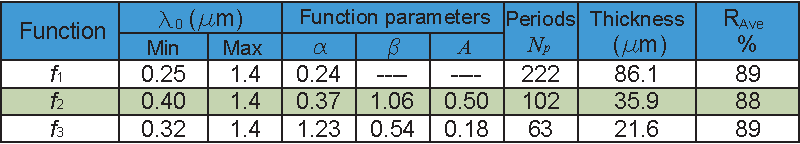
\includegraphics[width=\textwidth]
{F2TableOptimized.pdf}
\end{table}

According to the values shown in table I, the structure (named as ST-A) that has the
maximum average reflectance with the minimum thickness is the one designed
with the function $f_{3}$ (Eq. (\ref{F3})). Thus, the first and last periods
are tuned to 320 and 1400 nm, respectively. The complete distribution of the
periods is presented in Fig. \ref{Fig2}(a).
\begin{figure}
\begin{center}
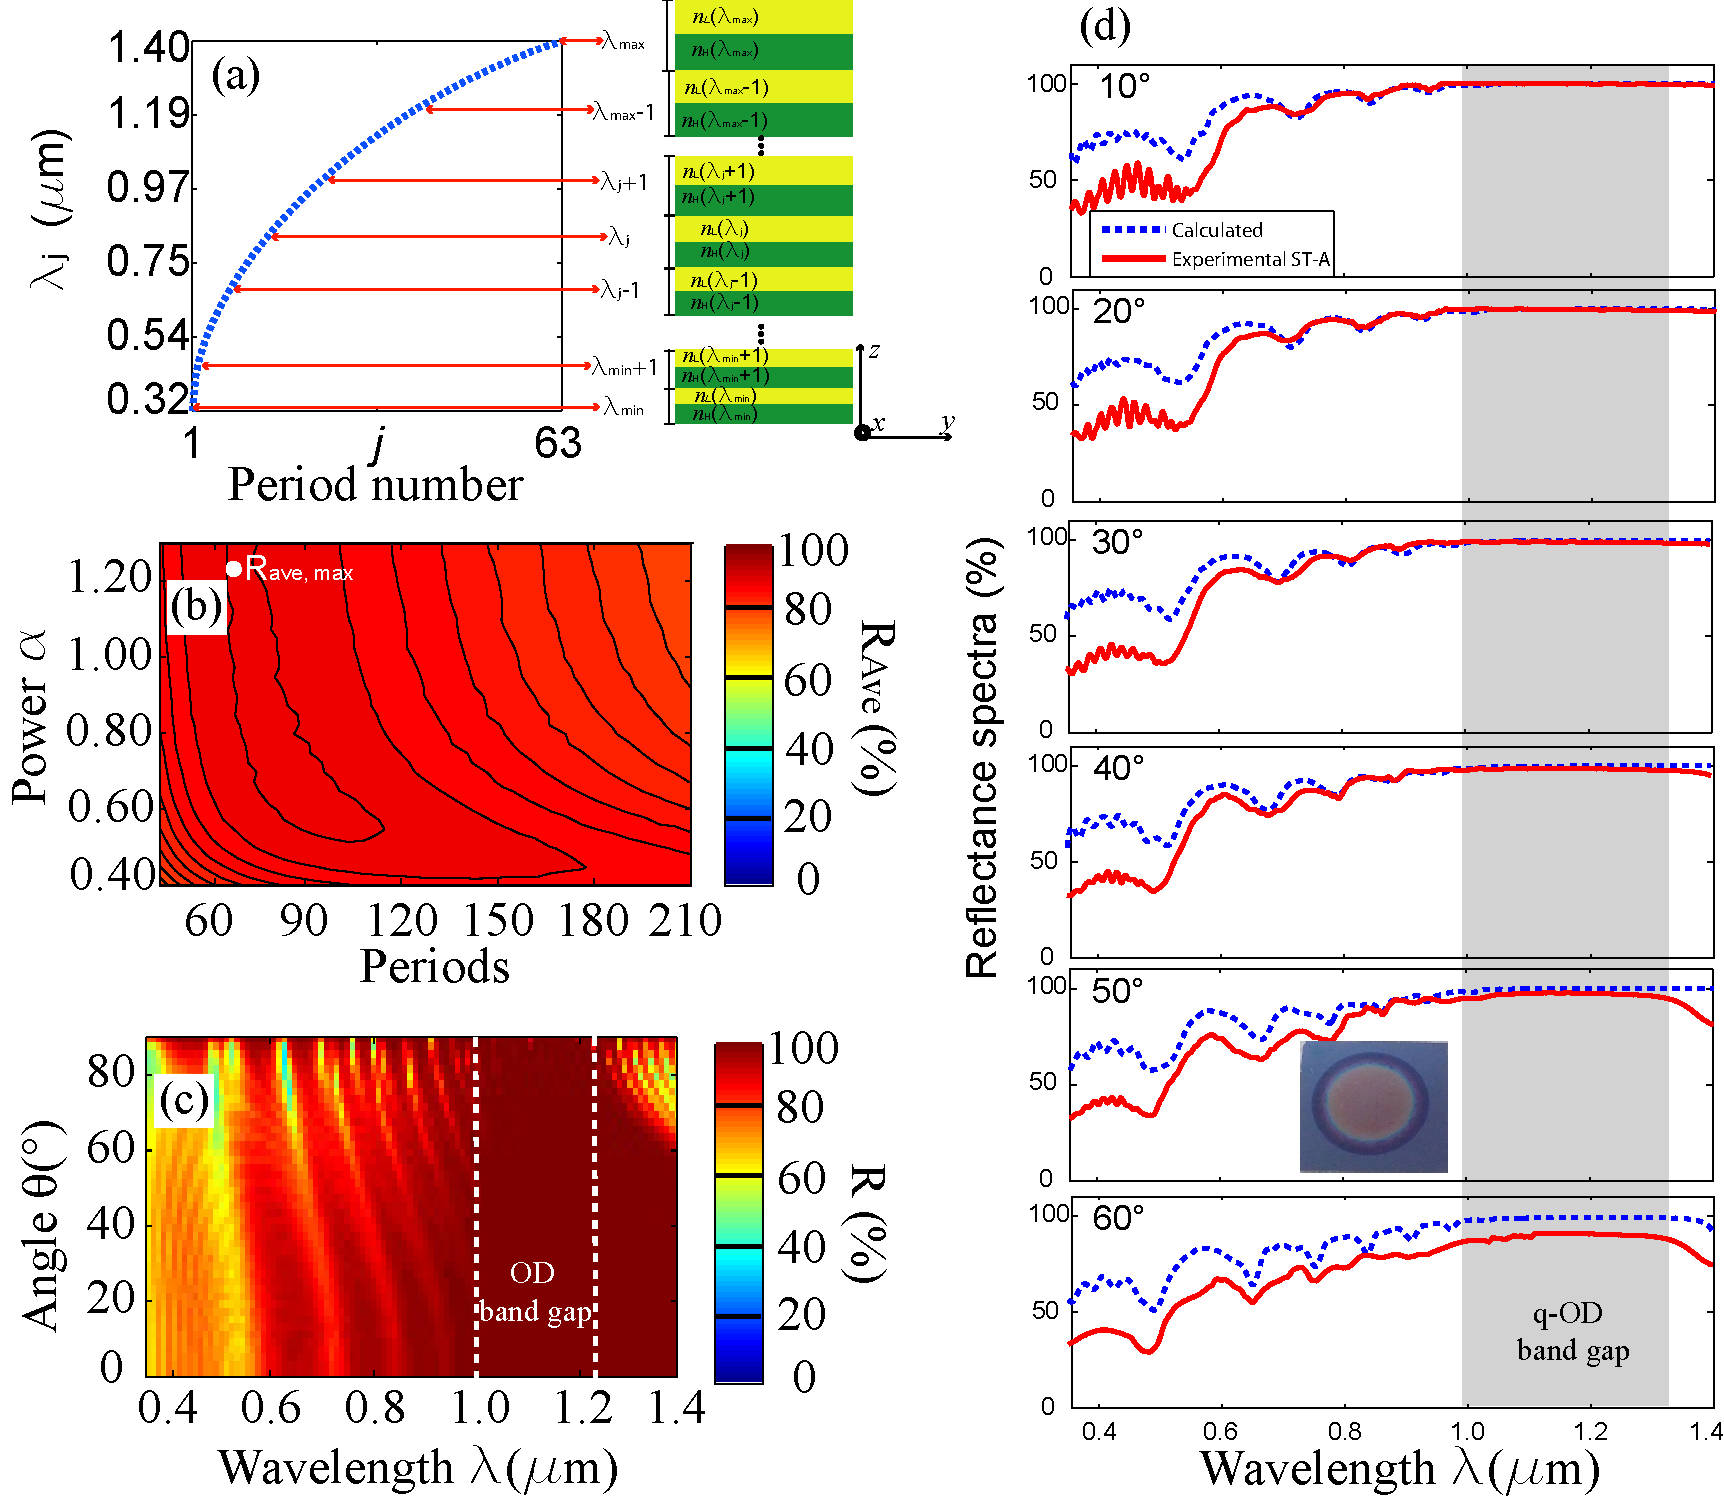
\includegraphics[width=\textwidth]
		{F3OptimizedVis.pdf}
\end{center}
\caption{(a) Distribution of $\protect\lambda _{j}$ in the $j$-th period for
the design of the 63-period multilayer structure. (b) Mapping of the average
reflectance of the structures designed with different values{}of $%
\protect\alpha $ and $N_{p}$ parameters. It is verified that the parameters
obtained during the optimization are adequate ($\protect\alpha =1.23$ and $%
N_{p}=63$). (c) Mapping the calculated reflectance for non polarized light of the
designed structure with the optimized values. (d) Comparison of reflectance spectra
calculated and measured at different angles of incidence. The gray band indicates the
region in which the reflectance is greater than 95\%. Inset shows the
top view photograph of the synthesized structure.}
\label{Fig2}
\end{figure}
To verify that the values
obtained are optimal, in Fig. \ref{Fig2}(b), the average reflectances of the
photonic structures designed with different parameters are mapped and,
indeed, the values are in the area where R$_{\text{ave}}\left( \lambda
,\theta \right)$ is maximum. Here, the parameters $\lambda _{\text{min}}$,
$\lambda _{\text{max}}$, $\beta$ and $A$ were adjusted, while $N_{p}$ and $\alpha $
varied from 30 to 200 periods and from 0.4 to 1.3, respectively. The calculated
reflectance, R$\left( \lambda ,\theta \right) $, of the photonic structure is shown
in Fig \ref{Fig2}(c). Here, the wavelength and incidence angle cover the ranges
from 350 to 1400 nm, and from 0${{}^\circ}$ to 90${{}^\circ}$, respectively.
Calculations indicate that the structure has a localized omnidirectional band gap
from 1000 to 1200 nm, taken with a reflectance greater than 95$\%$. Due to
experimental limitations, reflectance spectra for non polarized light are shown in all results.
In Fig. \ref{Fig2}(d), the calculated and measured reflectance is compared
at 10${{}^\circ}$, 20${{}^\circ}$, 30${{}^\circ}$, 40${{}^\circ}$, 50${{}^\circ}$
and 60${{}^\circ}$ of incidence. In this angular range, the structure has a
quasi-omnidirectional band gap (R$\left(\lambda,\theta\right)>95\%$) located from
980 to 1340 nm. The numerical and experimental spectral line shapes at different
angles are in good agreement. For wavelengths greater than 700 nm and lying between
10${{}^\circ}$ to 40${{}^\circ}$ of incidence angle, the difference in spectra is
less than $5\%$. For angles of incidence greater than 40 degree, although their
characteristics are similar, the measured spectrum demonstrates relatively less
reflectance than calculated reflectance. This difference can be attributed, in part,
to the scattering of light between each of the actual interfaces, which generally
have some roughness \cite{Theiss1994,Chavez2020}.

Due to the absorptive nature of Si in the UV and visible region, it is relatively
difficult to design porous silicon omnidirectional mirrors in that region.
However, in the IR region, it is relatively easy to obtain highly reflective
and even omnidirectional photonic structures over a wide range. Therefore,
the average reflectance was optimized using the function $f_{1}$ (Eq. (\ref{F1}))
in the region of 850 to 3000 nm. It was found that the best value for
$\alpha $ is 1.2 and the minimum thickness is 60.4 $\mu$m, distributed in
90 periods. The complete design of the structure (named as ST-B) is graphed in Fig.
\ref{Fig3}(a).
\begin{figure}[tbph]
\begin{center}
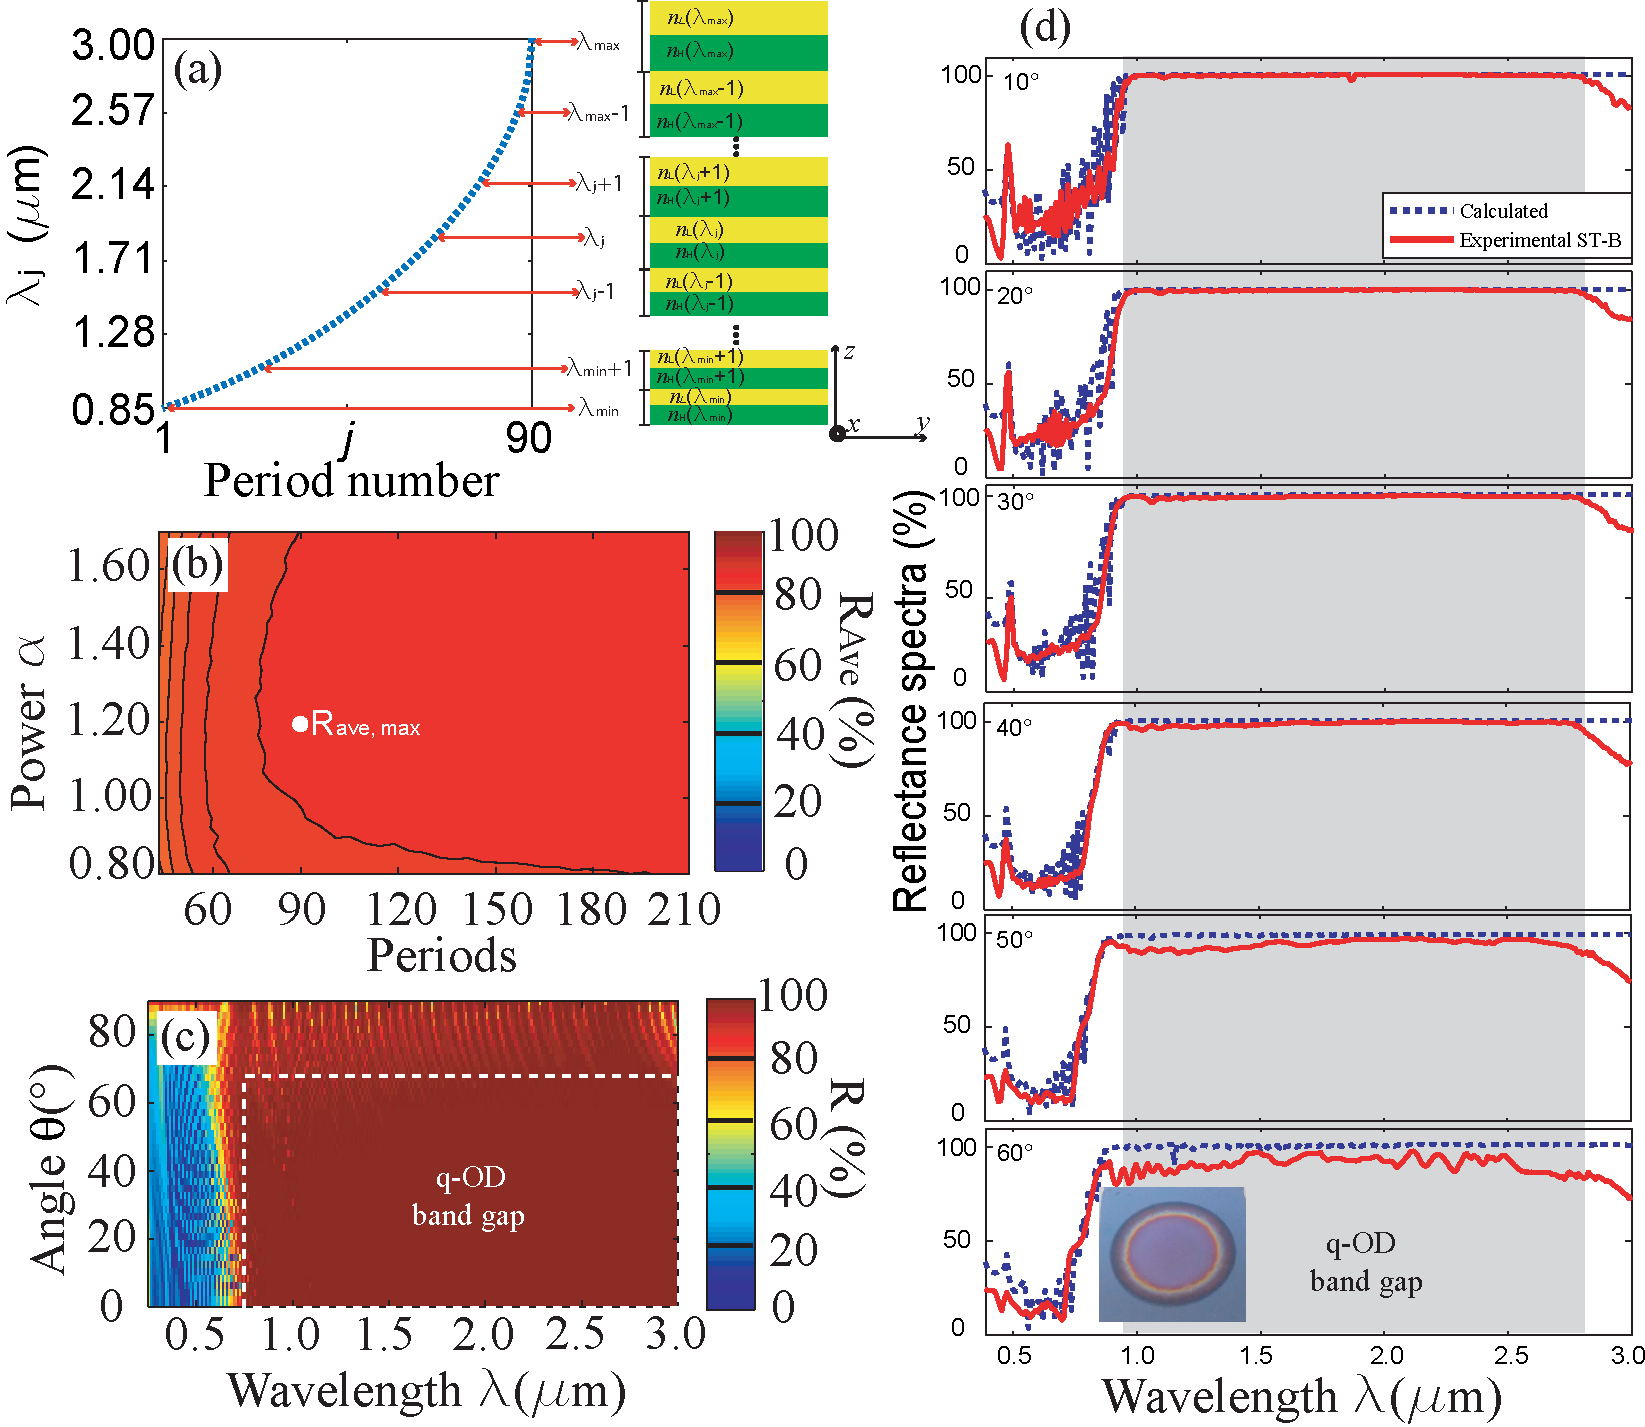
\includegraphics[width=\textwidth]
{F4OptimizedNIRPC.pdf}
\end{center}
\caption{(a) Distribution of $\protect\lambda _{j}$ in the $j$-th period
modulated by the optimization of the function $f_{1}$ for the design of the
multilayer structure of 90 periods. (b) Mapping of the average reflectance
of the structures designed with different values of the $\protect\alpha $
and $N_{p}$ parameters. The optimized parameters are $\protect\alpha =1.2$
and 90 periods. (c) Mapping the calculated reflectance of the designed
structure with the optimized values for non polarized light. (d) Comparison of
reflectance spectra calculated and measured at different angles of incidence. The
gray band indicates the region in which the reflectance is greater than 95$\%$. Inset
there is a photograph of the synthesized structure.}
\label{Fig3}
\end{figure}
In Fig \ref{Fig3}(b) the average reflectance of structures
designed with different values of $\alpha$ and $N_{p}$ is mapped. As in the
previous case, the optimized parameters are within the zone of maximum
average reflectance. The reflectance calculation shows that this structure
has a wide quasi-omnidirectional gap that goes from 850 to 3000 nm and from
0${{}^\circ}$ to 70${{}^\circ}$ of incidence; the corresponding contour plot is
shown in Fig. \ref{Fig3}(c) and its average reflectance between 850-3000nm is
greater than 95\%. The measured and calculated reflectance spectra have very
similar characteristics as shown in Fig \ref{Fig3}(d).  The synthesized PS
multilayered 1D photonic structure has a quasi omnidirectional (from 0${{}^\circ}$
to 60${{}^\circ}$) band gap of approximately 1800 nm. The difference
between the calculated and measured spectra at the longer wavelengths can be
attributed to a thickness gradient along the depth, which is more pronounced in
the lower layers due to the restricted diffusivity of the electrolyte
through the structure itself \cite{Negro2003,Vincent1993} and interface roughness.

\subsection{Photonic structure with sub-mirrors stacking}

Another technique to design Bragg mirrors in a wide range of the
electromagnetic spectrum is by stacking sub-mirrors at different
wavelengths \cite{Xifre20,DelRio2018,Agarwal2003}. Such grouping must meet the condition
imposed by the dispersion relation, $\cos KD=\frac{1}{2}\text{Tr}\,M$, where $D$ is
the period, which corresponds to the actual thickness of the sub-mirror, $\pm K$
represents a 1D Bloch's vector corresponding to a wave that propagates along
$z$-direction \cite{Mochan1987,Mochan1988,Perez2018}, and T$\text{r}$ denotes the
trace. This equation is bounded by the minimum and maximum values that the cosine
function can take. Furthermore, if  the value of $\left\vert \text{Tr}\left(
M\right) \right\vert$ is $>2$, it indicates that this frequency will not
be able to propagate through the structure.

The ideal stack of sub-mirrors would be that PBG of the $j$-th mirror begins
at the edge of the PBG of the $j-1$-th mirror, until the desired interval has been covered.
However, this arrangement does not give the maximum average reflectance due to the
decrease in the reflectance at each intersection of the two PBGs. On the other hand,
the number of periods of each sub-mirror is an important parameter due to its direct
dependence on the magnitude and  width of  the photonic band gap.  As the structures
were synthesized using porous silicon, it is essential to minimize the number of
periods corresponding to the visible region sub-mirrors. Also, in the supplementary
information we show the reflectance calculations for structures composed of sub
mirrors with a constant number of periods, in these cases ODBMs are not obtained.
For these reasons, the number of periods for each mirror was chosen as follows: for
design wavelengths less than 500 nm ($\lambda_{D}<$500 nm), one period, for 500
$<\lambda_{D}<$650 nm, two periods , for 650 $<\lambda_{D}<$800 nm, three, and for
$\lambda_{D}>$ 800 nm, the number of periods was variable (Fig. \ref{Fig4}(a)).
\begin{figure}[tbph]
\begin{center}
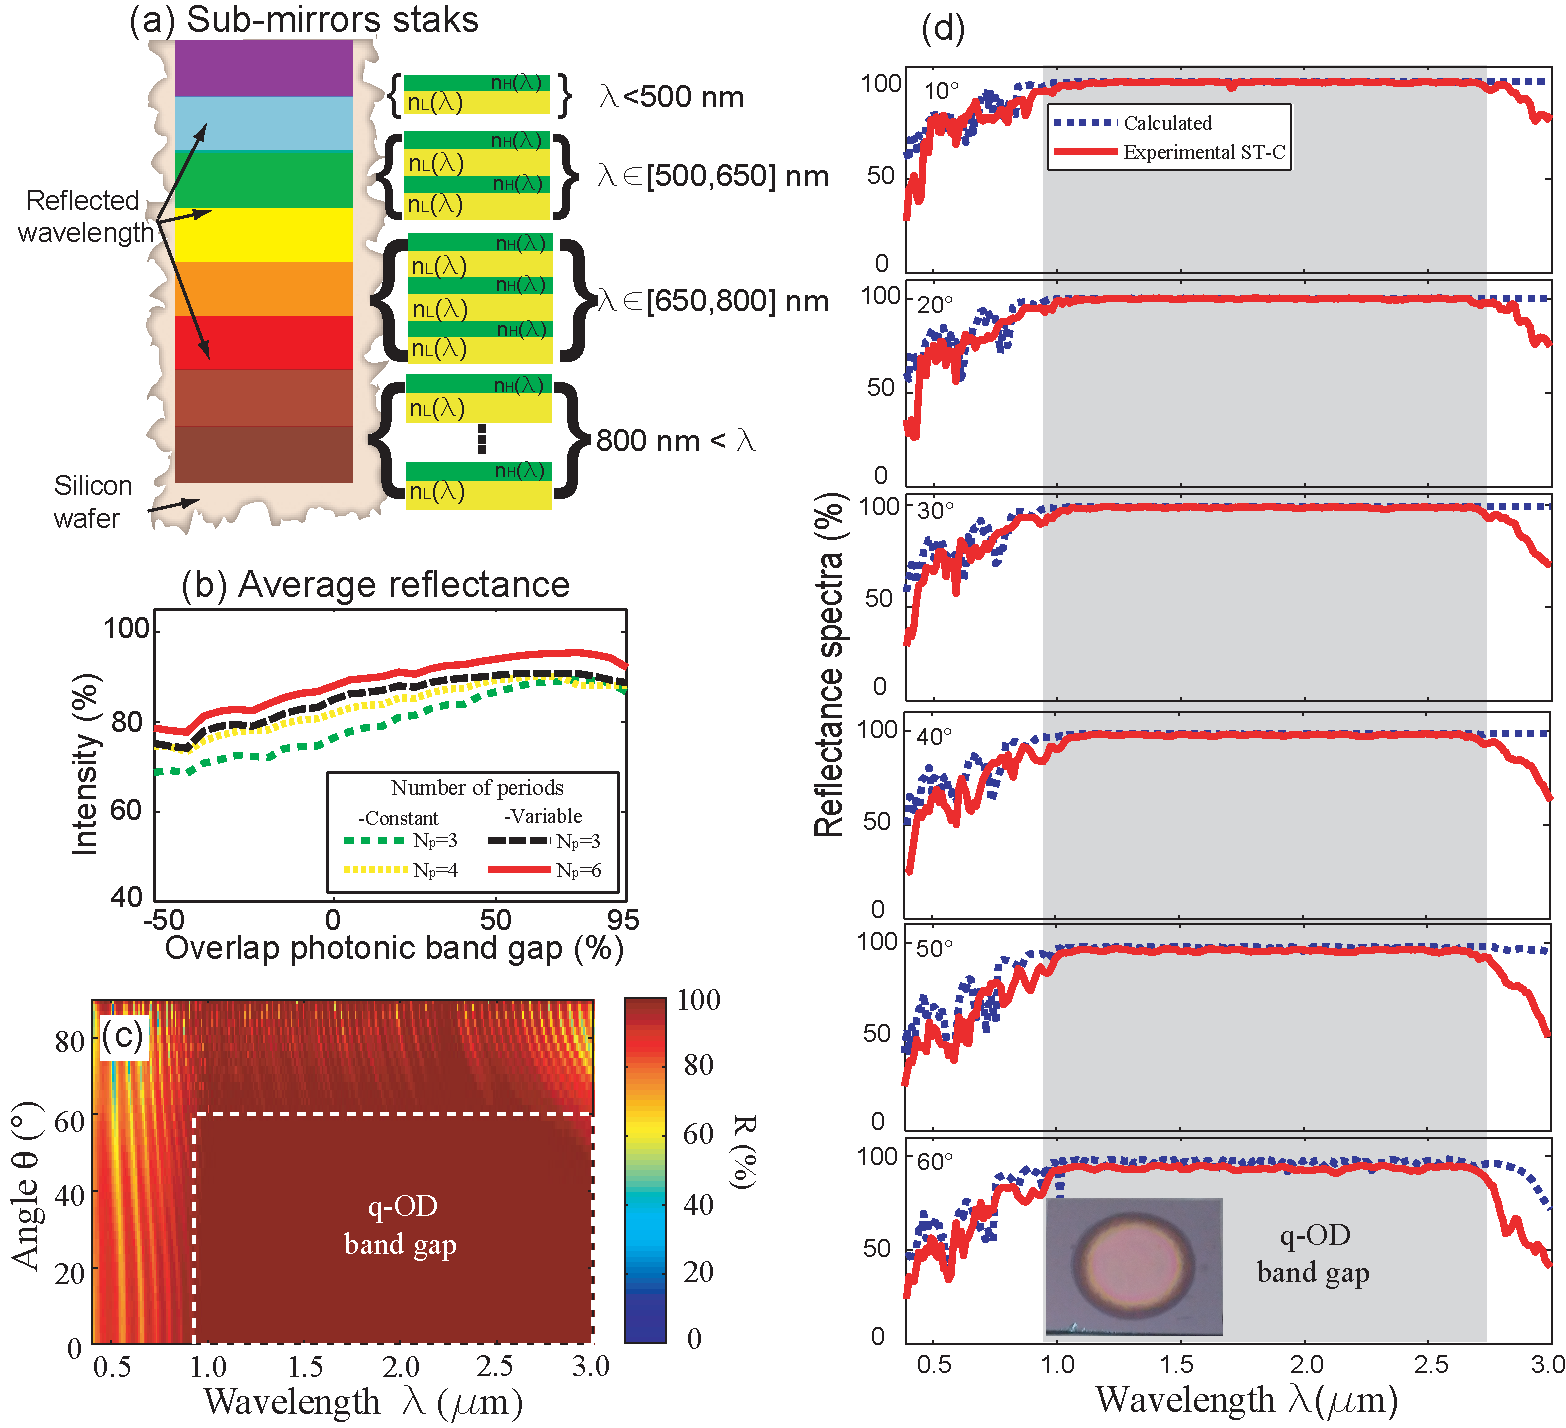
\includegraphics[width=\textwidth]
{F6OptimizedNIRSE.pdf}
\end{center}
\caption{(a) Diagram showing the distribution of sub-mirrors and the corresponding
number of periods in a PS multilayer. (b) Maximization of the average reflectance as
a function of the overlap photonic band gap for the structures formed by sub-mirrors
with a fixed number of periods (3 and 4), and for structures with the design of (a)
using 3 and 6 periods for the tuned sub-mirrors in $\lambda>800$ nm. (c) Mapping the
calculated reflectance of the designed structure with the optimized values for non
polarized light. (d) Comparison of reflectance spectra calculated and measured at
different angles of incidence. The gray band indicates the region in which the
reflectance is greater than 95$\%$. Inset shows the top view photograph of the
synthesized structure.}
\label{Fig4}
\end{figure}

Therefore, in this work the overlap percentage of the PBGs of the first and second
mirror, second and third mirror, and so on, is also optimized. Fig \ref{Fig4}(b)
shows the optimization results in terms of maximum average reflectance with respect
to the PBG overlap at different sub-mirror periods, keeping them fixed (3, 4) or
variable (1, 2  and 3) for $\lambda<500$(1 period), $500<\lambda<650$ nm (2
periods), $650<\lambda<800$ nm (3 periods) and $\lambda>800$ (3, 6 periods). For
example, the calculations corresponding to the reflectance spectra of the structures
formed using sub-mirrors with constant periods (3 and 4) revealed a lower average
reflectance as compared to the structure formed with variable periods. The 1D
photonic structure with the highest average reflectance (named as ST-C)  is the one
designed with variable periods and contemplates 6 periods for each sub-mirror in the
NIR region. In the optimized structure designed for 400-3000 nm range, the photonic
band gap overlap is around 78$\%$, thickness is 41.5 $\mu $m and the average
reflectance is 95.3$\%$, when the  electromagnetic waves are incident from
0${{}^\circ}$ to 89 ${{}^\circ}$. The optimized photonic structure is made up of 18
sub-mirrors tuned to the following wavelengths 400, 460, 510, 570, 640, 720,810,
910, 1020, 1150, 1290, 1450, 1630, 1830, 2060, 2320, 2610 and 2860 nm  with periods
of 1 (400, 460 nm), 2(510, 570, 640 nm), 3 (720 nm) and 6 (810 nm and above).

The reflectance mapping shown in Fig \ref{Fig4}(c) reveals a quasi omnidirectional
band gap from 950 to 2900 nm, taking into account 0${{}^\circ}$ to 60${{}^\circ}$ of
incidence. It is also observed that at incidence angles $>$70${{}^\circ}$, for long
wavelengths the reflectance decreases and has oscillations, which are attributed to
the greater penetration of the electromagnetic field within the structure, as shown
by Puente-D\'{\i}az, et al \cite{Puente2020}. Furthermore, in supplementary
information we show the transfer matrix trace calculations as a function of the
wavelength and the incidence angle for the ST-C photonic structure using the TE and
TM polarization. In Fig \ref{Fig4}(d) the calculated and measured reflectance
corresponding to the structure ST-C, at different angles of incidence is compared.
Although, the quasi omnidirectional band gap of the synthesized structure is
slightly less than that calculated (located from 950 to 2750 nm), the measured PBG
is almost twice as compared to the recently reported similar structures
(\cite{DelRio2018,Chavez2020}).

Finally, table 2 shows some porous silicon based ODBMs designed to operate in the
NIR region and the width of the omnidirectional band gap is compared with the
structures analyzed in the present study. The table reveals that the porous silicon
based structures ST-B and ST-C have the widest gap width, being 1.8 times greater
than recently reported works.

\begin{table}[h!]
	\begin{center}
		\caption{Summary of the development in porous silicon based ODBMs designed in the NIR region.}
		\label{tab:table1}
		\begin{tabular}{c|c|c|c}
			\hline % <-- Toprule here
		\textbf{Reference}&\textbf{Year}&\textbf{ODBM range}&\textbf{ODBM width}\\
			%\multicolumn{3}{c|}{\textbf{ODBM width}} \\ % <-- Combining two cells with alignment c| and content 12.
			 & &(nm)&(nm)\\%&\textbf{ST-B}&\textbf{ST-C}\\
			\hline % <-- Midrule here
Bruyant, et al \cite{Bruyant2003}. & 2003 & 1100-1440 & 340 \\
Xifre-P\'{e}rez, et al \cite{Xifre2005}. & 2004 & 1297-1615 & 318\\
Estevez, et al \cite{Estevez2009}. & 2009 & 950-1456 & 506 \\
Chavez, et al \cite{Chavez2020}. & 2020 & 1000-2000 & 1000 \\
			\hline % <-- Bottomrule here
			\begin{tabular}{c|c}
					&ST-A\\
					This article&ST-B\\
				&ST-C\\
			\end{tabular}&
			\begin{tabular}{c}
			\\
			\\
			\\
			\end{tabular}&
		\begin{tabular}{c}
			980-1340\\
			980-2780\\
			950-2750\\
		\end{tabular}&
		\begin{tabular}{c}
			360\\
			1800\\
			1800\\
		\end{tabular}\\
		\hline % <-- Bottomrule here
	\end{tabular}
	\end{center}
\end{table}


\section{Conclusion}

We have demonstrated the formation of highly reflective PS multilayer photonic
structures optimized using two types of design techniques for maximal reflectance
and minimal thickness in the NIR region. With \textit{chirped}-type Bragg mirrors,
two regions of the electromagnetic spectrum were analyzed. The first region (350nm -
1400 nm), optimized through an increasing function resulted in an average
reflectance $>85\%$ with the quasi omnidirectional PBG of 360 nm centered at 1160 nm
(980-1340 nm) for the angular range 0-60${{}^\circ}$ and more than 50$\%$ of
reflectance from 550-980nm. The second structure was designed for 850-3000 nm
wavelength range and the synthesized structure with optimized parameters resulted in
the average reflectance of $~91\%$ with q-OD bandgap from 980 to 2780 nm and a
thickness of 60.4 $\mu$m. The other design technique consisting of sub-mirrors
stacks (designed at different wavelengths), was optimized for maximum average
reflectance with respect to the percentage overlap of the PBG for each sub-mirror. A
multilayer structure using the optimized parameters with sub-mirrors stack method
was obtained with the average reflectance of $~95\%$ and a thickness of 41.5 $\mu$m.
Furthermore, this structure revealed a 1800 nm q-OD PBG, centered at 1850 nm, in
angular range 0-60${{}^\circ}$. Therefore, this second technique was found to be
better due to the decreased thickness (by a factor of $~1.5$) of the framework and
increased average reflectance. Additionally, the analysis techniques developed here
can be used to optimize reflectance with other refractive index contrasts in PS
multilayers or different other systems composed of other types of materials. Such
proposed structures could be used as mirrors for solar concentrators, flat focusing reflectors,
 thermal regulators, or, if defects are included, as filters or remote chemical/biosensors
with a wide angular independent response.



\section*{Acknowledgments}
This work was partially supported by Consejo Nacional de Ciencia y Tecnolog\'{i}a through grant No. \textbf{256243} and C\'{a}tedras Conacyt program 1577.
%\end{acknowledgments}


\begin{thebibliography}{99}
\bibitem{Joannopoulos2008} J. D. Joannopoulos et al., Photonic Crystals:
Molding the Flow of Light, Princeton University Press, New Jersey (2008).

\bibitem{Goyal2018} A. K. Goyal et al., Porous photonic crystal structure
for sensing applications,\ \textit{J. Nanophotonics }12(\textbf{4}), 040501
(2018).

\bibitem{Lopez2013} C. L\'{o}pez, Materials aspects of photonic crystals,
\textit{Adv. Mater.} \textbf{15}, 1679--1704 (2013).

\bibitem{Masaya2010} N. Masaya, Manipulating light with strongly modulated
photonic crystals, \textit{Rep. Prog.Phys.} \textbf{73} 096501, (2010).

\bibitem{Kumar2020} A. K. Goyal, A. Kumar, Recent advances and progresses in
photonic devices for passive radiative cooling application: a review,
\textit{J. Nanophoton}. 14(\textbf{3}) 030901 (2020)
https://doi.org/10.1117/1.JNP.14.030901

\bibitem{Zipock1997} R. Szip\"{o}cs and A. Koh\'{a}zi-Kis, Theory and design
of chirped dielectric mirrors, \textit{Appl. Phys. B }\textbf{65}, 115
(1997), doi:10.1007/s003400050258

\bibitem{Xifre2009} Xifre-Perez, Appl Phys B, 95: 169-172 (2009)

\bibitem{Chen1999} K.M. Chen, A.W. Sparks, H.-C. Luan, D.R. Lim, K.Wada,
L.C. Kimerling, SiO2/TiO2 omnidirectional reflector andmicrocavity resonator
via the sol--gelmethod, \textit{Appl. Phys. Lett. 75}  3805--3807, (1999).

\bibitem{Park2003} Y. Park, Y.-G. Roh, C.-O. Cho, H. Jeon, M.G. Sung,
J.C.Woo, GaAs-based near-infrared omnidirectional reflector, \textit{Appl.
Phys. Lett}. \textbf{82} (2003) 2770--2772.

\bibitem{DeCorby2005} R. G. DeCorby, H. T. Nguyen, P. K. Dwivedi, and T. J.
Clement, Planar omnidirectional reflectors in chalcogenide glass and
polymer, \textit{Opt. Express }13, 6228-6233 (2005)

\bibitem{Jena2016} S. Jena, R.B. Tokas, S. Tripathi, K.D. Rao, D.V. Udupa,
S. Thakur, N.K. Sahoo Influence of oxygen partial pressure on
microstructure, optical properties, residual stress and laser induced damage
threshold of amorphous HfO2 thin films \textit{Journal of Alloys and
Compounds}, Volume 771, 2019, pp. 373-381

\bibitem{Xifre2015} Xifr\'{e}-P\'{e}rez E., Ferr\'{e}-Borrull J., Pallar\'{e}%
s J., and Marsal L. F. Methods, Properties and Applications of Porous
Silicon, \textit{Electrochemically Engineered Nanoporous Materials},
Springer Series in Materials Science 220, Ch.2, (2015).

\bibitem{Pavesi2000} Bisi O., Stefano Ossicini, and Pavesi L. Porous
silicon: a quantum sponge structure for silicon based optoelectronics,
\textit{Surface Science Reports} \textbf{38} 1-126, (2000).

\bibitem{Estevez2009} Estevez J. O., Arriaga J., M\'{e}ndez Blas A., and
Agarwal V. Enlargement of omnidirectional photonic band gap in porous silicon
dielectric mirrors with a Gaussian profile refractive index. \textit{Applied
Physics Lettesrs}, \textbf{94}, 061914, (2009).

\bibitem{Ariza2014} Ariza-Flores D., P\'{e}rez-Huerta J.S., Kumar Y.,
Encinas A., and Agarwal V. Design and optimization of antireflecting
coatings from nanostructured porous silicon dielectric multilayers. \textit{%
Solar Energy Materials \& Solar Cells}, \textbf{123} 144-149, (2014).

\bibitem{Giusseppe2011} Ruminski A.M., Barillaro G., Chaffin C., and Sailor
M. J., Internally Referenced Remote Sensors for HF and Cl2 Using Reactive
Porous Silicon Photonic Crystals. \textit{Adv. Funct. Mater.}, \textbf{21}:
1511-1525, (2011).

\bibitem{Agarwal2018} Karthik T.V.K., Martinez L., and Agarwal V. Porous
silicon ZnO/SnO$_{2}$ structures for CO$_{2}$ detection. \textit{Journal of
Allows and Compounds}, \textbf{731} 853-863, (2018).

\bibitem{Hussel1997} C.P. Hussell, R.V. Ramaswamy, \textit{IEEE Photonics
Technol. Lett.} \textbf{9}, 636, (1997).

\bibitem{Antunez2014} Antunez E.E., Estevez J.O., Campos J., Basurto-Pensado
M.A., and V.Agarwal V. Formation of photoluminescent n-type macroporous
silicon: Effect of magnetic field and lateral electric potential. \textit{%
Physica B} \textbf{453} 34--39, (2014).

\bibitem{Kozar2017} A. V. Kozar, S. V. Marchenko and P. Y. Shestakov, "Focusing and defocusing of reflected light beams from chirped dielectric layered structure," 2017 Days on Diffraction (DD), St. Petersburg, pp. 200-204, (2017).

\bibitem{Cheng2018} Yu-Chieh Cheng and  Kestutis Staliunas, Near-field flat focusing mirrors, Applied Physics Reviews 5, 011101 (2018).

\bibitem{Jimenez2020} Jimen\'{e}z-Vivanco M. R., Garc\'{\i}a G., Carrillo
J., Agarwal V., D\'{\i}az-Becerril T., Doti R., Faubert J., and Lugo J. E.
Porous Si-SiO2 based UV Microcavities. \textit{Scientific Reports} \textbf{10%
}: 2220, (2020).

\bibitem{Ariza2012} Ariza-Flores A. D., Gaggero-Sager L. M., and Agarwal V.
White metal like omnidirectional mirror from porous silicon dielectric
multilayers. \textit{Appl. Phys. Lett.}, 101(\textbf{3}):031119, (2012).

\bibitem{Bruyant2003} Bruyant A., L erondel G., Reece P. J., and Gal M.
All-silicon omnidirectional mirrors based on one-dimensional photonic
crystals. \textit{Appl. Phys. Lett.}, 82(\textbf{19}):3227-3229, (2003).

\bibitem{DelRio2018} Estrada-Wiese, D., del R\'{\i}o-Chanona, E.A. \& del R%
\'{\i}o, J.A. Stochastic optimization of broadband reflecting photonic
structures. \textit{Sci Rep} \textbf{8}, 1193 (2018).

\bibitem{Chavez2020} B. A. Chavez-Castillo, J. S. P\'{e}rez-Huerta, J.
Madrigal-Melchor, S. Amador-Alvarado, I. A. Sustaita-Torres, V. Agarwal, and
D. Ariza-Flores, A wide band porous silicon omnidirectional mirror for the
near infrared range, \textit{Journal of Applied Physics}, \textbf{127}, 20,
(2020).

\bibitem{Mochan1987} Moch\'{a}n W. L., del Castillo-Mussot M., and Barrera
Rub\'{e}n G. Effect of plasma waves on the optical properties of
metal-insulator superlattices. \textit{Phys. Rev. B}, 35(\textbf{3}%
):1088-1098, (1987).

\bibitem{Ortiz2020} Leandro L. Missoni, Guillermo P. Ortiz, Mar\'{i}a Luz
Mart\'{\i}nez Ricci, Victor J. Toranzos, W. Luis Moch\'{a}n, Rough 1D
photonic crystals: A transfer matrix approach, \textit{Optical Materials},
\textbf{109}, 110012 (2020).

\bibitem{Puente2020} Luis Eduardo Puente-D\'{i}az, Victor
Castillo-Gallardo, Guillermo P. Ortiz, Jos\'{e} Samuel P\'{e}rez-Huerta, H%
\'{e}ctor P\'{e}rez-Aguilar, Vivechana Agarwal, W. Luis Moch\'{a}n, Stable
calculation of optical properties of large non-periodic dissipative
multilayered systems, \textit{Superlattices and Microstructures}, \textbf{145%
}, 106629, (2020).

\bibitem{Pap2006} Pap Andrea Edit, Kord\'{a}s Kriszti\'{a}n, V\"{a}h\"{a}kangas
Jouko, Uusim\"{a}ki Antti, Lepp\"{a}vuori Seppo, Pilon Laurent, and Szatm\'{a}ri
S\'{a}ndor. Optical properties of porous silicon. part iii: Comparison of
experimental and theoretical results. \textit{Optical Materials}, 28(5):506-513, (2006).

\bibitem{Estrada2018} D. Estrada-Wiese and J. A. del R\'{\i}o, Refractive index evaluation of porous silicon using Bragg reflectors. \textit{Revista mexicana de f\'{\i}sica}, \textbf{64}(1), 72-81, (2018).

\bibitem{minuit} James F. and Winkler M. Minuit user's guide. CERN, Geneva,
(2004).

\bibitem{Canham90} Canham L. T. Silicon quantum wire array fabrication by
electrochemical and chemical dissolution of wafers. \textit{Appl. Phys. Lett.%
}, 57(\textbf{10}):1046-1048, (1990).

\bibitem{Escorcia07} Escorcia J. and Agarwal V. E ect of duty cycle and
frequency on the morphology of porous silicon formed by alternating square
pulse anodic etching. \textit{Phys. Status Solidi (c)}, 4(\textbf{6}%
):2039-2043, (2007).

\bibitem{Ariza2011} A. David Ariza-Flores, L M Gaggero-Sager and V Agarwal,
Effect of interface gradient on the optical properties of multilayered porous
silicon photonic structures, J Phys D: Appl Phys, 44(15), 155102 (2011)

\bibitem{Brugeman2006} Andrea Edit Pap, Kriszti an Kord as, Jouko
Vahakangas, Antti Uusimaki, Seppo Leppavuori, Laurent Pilon, and Sandor
Szatmari. Optical properties of porous silicon. part iii: Comparison of
experimental and theoretical results. \textit{Optical Materials}, 28(\textbf{%
5}):506-513, (2006).

\bibitem{Theiss1994} W. Thei\ss , R. Arens-Fischer, M. Arntzen, M.G. Berger,
S. Frohnhoff, S. Hilbrich, andWernke M. Probing optical transitions in
porous silicon by reflectance spectroscopy in the near infrared, visible and
UV. \textit{MRS Proceedings}, 358:435, (1994).

\bibitem{Negro2003} L. Dal Negro, C. J. Oton, Z. Gaburro, L. Pavesi, P.
Johnson, A. Lagendijk, R. Righini, M. Colocci, and D. S. Wiersma. Light
Transport through the Band-Edge States of Fibonacci Quasicrystals. \textit{%
	Phys. Rev. Lett}. \textbf{90}, 055501, (2003).

\bibitem{Vincent1993} G. Vincent. Optical properties of porous silicon
superlattices \textit{Appl. Phys. Lett}. \textbf{64}, 2367 (1994).

\bibitem{Agarwal2003} V. Agarwal and J. A. del R\'{\i}o, Tailoring the
photonic band gap of a porous silicon dielectric mirror, Applied Physics
Letters \textbf{82}, 1512 (2003).

\bibitem{Mochan1988} Moch\'{a}n W. L. and del Castillo-Mussot M. Optics of
multilayered conducting systems: Normal modes of periodic superlattices.
\textit{Phys. Rev. B}, 37(\textbf{12}):6763-6771, (1988).

\bibitem{Perez2018} P\'{e}rez-Huerta J. S., Ariza-Flores D., Castro-Garc%
\'{\i}a R., Moch\'{a}n W. L., Ortiz G. P., and Agarwall V. Reflectivity of
1D photonic crystals: A comparison of computational schemes with
experimental results. \textit{Int. J. Mod. Phys. B}, 32(\textbf{11}%
):1850136, (2018).

\bibitem{Xifre2005} E. Xifr\'{e}-P\'{e}rez, L. Marsal, J. Pallar\'{e}s, and
J. Ferr\'{e}-Borrull, \textquotedblleft Porous silicon mirrors with enlarged
omnidirectional band gap,\textquotedblright\ \textit{J. Appl. Phys.} \textbf{%
97}, 064503 (2005).

\bibitem{Estevez2005} Estevez J. O., Arriaga J., M\'{e}ndez Blas A., and
Agarwal V. Omnidirectional photonic band gaps in porous silicon based mirrors
with a Gaussian profile refractive index. \textit{Appl. Phys. Lett.} \textbf{%
93}:191915, (2005).


\end{thebibliography}

\end{document}
